\documentclass[twoside]{book}

% Packages required by doxygen
\usepackage{fixltx2e}
\usepackage{calc}
\usepackage{doxygen}
\usepackage[export]{adjustbox} % also loads graphicx
\usepackage{graphicx}
\usepackage[utf8]{inputenc}
\usepackage{makeidx}
\usepackage{multicol}
\usepackage{multirow}
\PassOptionsToPackage{warn}{textcomp}
\usepackage{textcomp}
\usepackage[nointegrals]{wasysym}
\usepackage[table]{xcolor}

% Font selection
\usepackage[T1]{fontenc}
\usepackage[scaled=.90]{helvet}
\usepackage{courier}
\usepackage{amssymb}
\usepackage{sectsty}
\renewcommand{\familydefault}{\sfdefault}
\allsectionsfont{%
  \fontseries{bc}\selectfont%
  \color{darkgray}%
}
\renewcommand{\DoxyLabelFont}{%
  \fontseries{bc}\selectfont%
  \color{darkgray}%
}
\newcommand{\+}{\discretionary{\mbox{\scriptsize$\hookleftarrow$}}{}{}}

% Page & text layout
\usepackage{geometry}
\geometry{%
  a4paper,%
  top=2.5cm,%
  bottom=2.5cm,%
  left=2.5cm,%
  right=2.5cm%
}
\tolerance=750
\hfuzz=15pt
\hbadness=750
\setlength{\emergencystretch}{15pt}
\setlength{\parindent}{0cm}
\setlength{\parskip}{3ex plus 2ex minus 2ex}
\makeatletter
\renewcommand{\paragraph}{%
  \@startsection{paragraph}{4}{0ex}{-1.0ex}{1.0ex}{%
    \normalfont\normalsize\bfseries\SS@parafont%
  }%
}
\renewcommand{\subparagraph}{%
  \@startsection{subparagraph}{5}{0ex}{-1.0ex}{1.0ex}{%
    \normalfont\normalsize\bfseries\SS@subparafont%
  }%
}
\makeatother

% Headers & footers
\usepackage{fancyhdr}
\pagestyle{fancyplain}
\fancyhead[LE]{\fancyplain{}{\bfseries\thepage}}
\fancyhead[CE]{\fancyplain{}{}}
\fancyhead[RE]{\fancyplain{}{\bfseries\leftmark}}
\fancyhead[LO]{\fancyplain{}{\bfseries\rightmark}}
\fancyhead[CO]{\fancyplain{}{}}
\fancyhead[RO]{\fancyplain{}{\bfseries\thepage}}
\fancyfoot[LE]{\fancyplain{}{}}
\fancyfoot[CE]{\fancyplain{}{}}
\fancyfoot[RE]{\fancyplain{}{\bfseries\scriptsize Generated by Doxygen }}
\fancyfoot[LO]{\fancyplain{}{\bfseries\scriptsize Generated by Doxygen }}
\fancyfoot[CO]{\fancyplain{}{}}
\fancyfoot[RO]{\fancyplain{}{}}
\renewcommand{\footrulewidth}{0.4pt}
\renewcommand{\chaptermark}[1]{%
  \markboth{#1}{}%
}
\renewcommand{\sectionmark}[1]{%
  \markright{\thesection\ #1}%
}

% Indices & bibliography
\usepackage{natbib}
\usepackage[titles]{tocloft}
\setcounter{tocdepth}{3}
\setcounter{secnumdepth}{5}
\makeindex

% Hyperlinks (required, but should be loaded last)
\usepackage{ifpdf}
\ifpdf
  \usepackage[pdftex,pagebackref=true]{hyperref}
\else
  \usepackage[ps2pdf,pagebackref=true]{hyperref}
\fi
\hypersetup{%
  colorlinks=true,%
  linkcolor=blue,%
  citecolor=blue,%
  unicode%
}

% Custom commands
\newcommand{\clearemptydoublepage}{%
  \newpage{\pagestyle{empty}\cleardoublepage}%
}

\usepackage{caption}
\captionsetup{labelsep=space,justification=centering,font={bf},singlelinecheck=off,skip=4pt,position=top}

%===== C O N T E N T S =====

\begin{document}

% Titlepage & ToC
\hypersetup{pageanchor=false,
             bookmarksnumbered=true,
             pdfencoding=unicode
            }
\pagenumbering{roman}
\begin{titlepage}
\vspace*{7cm}
\begin{center}%
{\Large Search folder }\\
\vspace*{1cm}
{\large Generated by Doxygen 1.8.11}\\
\end{center}
\end{titlepage}
\clearemptydoublepage
\tableofcontents
\clearemptydoublepage
\pagenumbering{arabic}
\hypersetup{pageanchor=true}

%--- Begin generated contents ---
\chapter{Data Structure Index}
\section{Data Structures}
Here are the data structures with brief descriptions\+:\begin{DoxyCompactList}
\item\contentsline{section}{\hyperlink{structfile__t}{file\+\_\+t} \\*Hashtable entry type used in {\ttfamily files} }{\pageref{structfile__t}}{}
\item\contentsline{section}{\hyperlink{structfinder__t}{finder\+\_\+t} \\*A chained list of found file names }{\pageref{structfinder__t}}{}
\item\contentsline{section}{\hyperlink{structio__file__list}{io\+\_\+file\+\_\+list} \\*Container for file lists (fixed size for simplification), used by \hyperlink{io_8c_adb8d68b54b043f5118a4cbfd49a8ec51}{io\+\_\+directory\+\_\+get\+\_\+all()} }{\pageref{structio__file__list}}{}
\item\contentsline{section}{\hyperlink{structparser__t}{parser\+\_\+t} \\*Formal expression representation }{\pageref{structparser__t}}{}
\item\contentsline{section}{\hyperlink{structsearchfolder__t}{searchfolder\+\_\+t} }{\pageref{structsearchfolder__t}}{}
\end{DoxyCompactList}

\chapter{File Index}
\section{File List}
Here is a list of all documented files with brief descriptions\+:\begin{DoxyCompactList}
\item\contentsline{section}{{\bfseries finder.\+c} }{\pageref{finder_8c}}{}
\item\contentsline{section}{{\bfseries finder.\+h} }{\pageref{finder_8h}}{}
\item\contentsline{section}{\hyperlink{io_8c}{io.\+c} \\*Helpers function around system calls for IO purpose }{\pageref{io_8c}}{}
\item\contentsline{section}{\hyperlink{io_8h}{io.\+h} \\*Helpers function around system calls for IO purpose }{\pageref{io_8h}}{}
\item\contentsline{section}{\hyperlink{ipc_8c}{ipc.\+c} \\*Manage communication between different instance of smartfolder }{\pageref{ipc_8c}}{}
\item\contentsline{section}{\hyperlink{ipc_8h}{ipc.\+h} \\*Manage communication between different instance of smartfolder }{\pageref{ipc_8h}}{}
\item\contentsline{section}{\hyperlink{linker_8c}{linker.\+c} \\*The linker maintains an updated list of links to the found files }{\pageref{linker_8c}}{}
\item\contentsline{section}{\hyperlink{linker_8h}{linker.\+h} \\*The linker maintains an updated list of links to the found files }{\pageref{linker_8h}}{}
\item\contentsline{section}{\hyperlink{logger_8c}{logger.\+c} \\*Simple logger functions that allow logging of various informations and errors }{\pageref{logger_8c}}{}
\item\contentsline{section}{\hyperlink{logger_8h}{logger.\+h} \\*Simple logger functions that allow logging of various informations and errors }{\pageref{logger_8h}}{}
\item\contentsline{section}{\hyperlink{main_8c}{main.\+c} \\*Main program\+: deamonise, parse argument and launch the search }{\pageref{main_8c}}{}
\item\contentsline{section}{\hyperlink{parser_8c}{parser.\+c} \\*Parses a string expression and return a formal representation }{\pageref{parser_8c}}{}
\item\contentsline{section}{\hyperlink{parser_8h}{parser.\+h} \\*Parses a string expression and return a formal representation }{\pageref{parser_8h}}{}
\item\contentsline{section}{{\bfseries searchfolder.\+c} }{\pageref{searchfolder_8c}}{}
\item\contentsline{section}{{\bfseries searchfolder.\+h} }{\pageref{searchfolder_8h}}{}
\item\contentsline{section}{\hyperlink{validator_8c}{validator.\+c} \\*Critera and operator evaluation functions }{\pageref{validator_8c}}{}
\item\contentsline{section}{\hyperlink{validator_8h}{validator.\+h} \\*Validates files against a parsed criteria expression }{\pageref{validator_8h}}{}
\end{DoxyCompactList}

\chapter{Data Structure Documentation}
\hypertarget{structfile__t}{}\section{file\+\_\+t Struct Reference}
\label{structfile__t}\index{file\+\_\+t@{file\+\_\+t}}
\subsection*{Data Fields}
\begin{DoxyCompactItemize}
\item 
long unsigned int {\bfseries id}\hypertarget{structfile__t_a44a772348760d7ca8095f707f652498a}{}\label{structfile__t_a44a772348760d7ca8095f707f652498a}

\item 
U\+T\+\_\+hash\+\_\+handle {\bfseries hh}\hypertarget{structfile__t_a67d3d81a4f9a9622b0befade8d131661}{}\label{structfile__t_a67d3d81a4f9a9622b0befade8d131661}

\end{DoxyCompactItemize}


\subsection{Detailed Description}


Definition at line 12 of file finder.\+c.



The documentation for this struct was generated from the following file\+:\begin{DoxyCompactItemize}
\item 
finder.\+c\end{DoxyCompactItemize}

\hypertarget{structfinder__t}{}\section{finder\+\_\+t Struct Reference}
\label{structfinder__t}\index{finder\+\_\+t@{finder\+\_\+t}}


A chained list of found file names.  




{\ttfamily \#include $<$finder.\+h$>$}



Collaboration diagram for finder\+\_\+t\+:\nopagebreak
\begin{figure}[H]
\begin{center}
\leavevmode
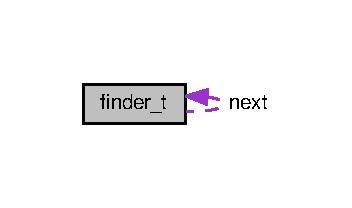
\includegraphics[width=188pt]{structfinder__t__coll__graph}
\end{center}
\end{figure}
\subsection*{Data Fields}
\begin{DoxyCompactItemize}
\item 
char $\ast$ \hyperlink{structfinder__t_aeac90097f29f7529968697163cea5c18}{filename}\hypertarget{structfinder__t_aeac90097f29f7529968697163cea5c18}{}\label{structfinder__t_aeac90097f29f7529968697163cea5c18}

\begin{DoxyCompactList}\small\item\em Found file name. \end{DoxyCompactList}\item 
struct \hyperlink{structfinder__t}{finder\+\_\+t} $\ast$ \hyperlink{structfinder__t_a7db9cac9324009990f14b7f84bf47d3c}{next}\hypertarget{structfinder__t_a7db9cac9324009990f14b7f84bf47d3c}{}\label{structfinder__t_a7db9cac9324009990f14b7f84bf47d3c}

\begin{DoxyCompactList}\small\item\em Next in the chain. \end{DoxyCompactList}\end{DoxyCompactItemize}


\subsection{Detailed Description}
A chained list of found file names. 

Definition at line 19 of file finder.\+h.



The documentation for this struct was generated from the following file\+:\begin{DoxyCompactItemize}
\item 
\hyperlink{finder_8h}{finder.\+h}\end{DoxyCompactItemize}

\hypertarget{structio__file__list}{}\section{io\+\_\+file\+\_\+list Struct Reference}
\label{structio__file__list}\index{io\+\_\+file\+\_\+list@{io\+\_\+file\+\_\+list}}
\subsection*{Data Fields}
\begin{DoxyCompactItemize}
\item 
char {\bfseries files} \mbox{[}I\+O\+\_\+\+D\+I\+R\+\_\+\+M\+A\+X\+\_\+\+F\+I\+L\+ES\mbox{]}\mbox{[}I\+O\+\_\+\+P\+A\+T\+H\+\_\+\+M\+A\+X\+\_\+\+S\+I\+ZE\mbox{]}\hypertarget{structio__file__list_aea2e7d487e7a0ce1737212bb7679dbcc}{}\label{structio__file__list_aea2e7d487e7a0ce1737212bb7679dbcc}

\item 
size\+\_\+t {\bfseries count}\hypertarget{structio__file__list_a76d971a3c552bc58ba9f0d5fceae9806}{}\label{structio__file__list_a76d971a3c552bc58ba9f0d5fceae9806}

\end{DoxyCompactItemize}


\subsection{Detailed Description}


Definition at line 17 of file io.\+h.



The documentation for this struct was generated from the following file\+:\begin{DoxyCompactItemize}
\item 
/home/claudio/git/smart-\/folder/src/io.\+h\end{DoxyCompactItemize}

\hypertarget{structparser__t}{}\section{parser\+\_\+t Struct Reference}
\label{structparser__t}\index{parser\+\_\+t@{parser\+\_\+t}}


Formal expression representation.  




{\ttfamily \#include $<$parser.\+h$>$}



Collaboration diagram for parser\+\_\+t\+:\nopagebreak
\begin{figure}[H]
\begin{center}
\leavevmode
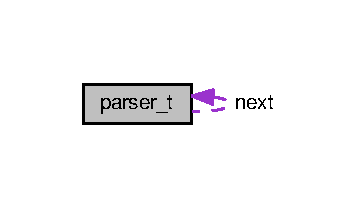
\includegraphics[width=172pt]{structparser__t__coll__graph}
\end{center}
\end{figure}
\subsection*{Data Fields}
\begin{DoxyCompactItemize}
\item 
\hyperlink{parser_8h_a4dcbe7148b91f50b0e7f3e08e780861d}{parser\+\_\+crit\+\_\+t} \hyperlink{structparser__t_af8e04406eee9097a92118be27b07eff7}{crit}
\begin{DoxyCompactList}\small\item\em The criteria for the token. \end{DoxyCompactList}\item 
void $\ast$ \hyperlink{structparser__t_a0f61d63b009d0880a89c843bd50d8d76}{value}
\begin{DoxyCompactList}\small\item\em The value of the criteria, the type depend on the type of \textquotesingle{}crit\textquotesingle{}. \end{DoxyCompactList}\item 
\hyperlink{parser_8h_ac721d0db2049edef01e62a2e63ff0472}{parser\+\_\+comp\+\_\+t} \hyperlink{structparser__t_a7bc05cec4ebb98215d11f1f354450f3d}{comp}
\begin{DoxyCompactList}\small\item\em The comparison to be used when evaluating the expression validity. \end{DoxyCompactList}\item 
struct \hyperlink{structparser__t}{parser\+\_\+t} $\ast$ \hyperlink{structparser__t_a044a5d882012dfdd9ea5e4f3a98fd8a2}{next}\hypertarget{structparser__t_a044a5d882012dfdd9ea5e4f3a98fd8a2}{}\label{structparser__t_a044a5d882012dfdd9ea5e4f3a98fd8a2}

\begin{DoxyCompactList}\small\item\em The next token in the expression. \end{DoxyCompactList}\end{DoxyCompactItemize}


\subsection{Detailed Description}
Formal expression representation. 

Contains the formal representation of the parsed expression in a ordered chained list. Each instance contains the information about a parsed expression token and the pointer to the {\ttfamily next} parsed expression token.

The order of the tokens in the chained list is not the same as the in the original string representation. Is has been reordered to encoded the priority of the operators and parenthesis in a infix notation 

Definition at line 71 of file parser.\+h.



\subsection{Field Documentation}
\index{parser\+\_\+t@{parser\+\_\+t}!comp@{comp}}
\index{comp@{comp}!parser\+\_\+t@{parser\+\_\+t}}
\subsubsection[{\texorpdfstring{comp}{comp}}]{\setlength{\rightskip}{0pt plus 5cm}{\bf parser\+\_\+comp\+\_\+t} comp}\hypertarget{structparser__t_a7bc05cec4ebb98215d11f1f354450f3d}{}\label{structparser__t_a7bc05cec4ebb98215d11f1f354450f3d}


The comparison to be used when evaluating the expression validity. 


\begin{DoxyItemize}
\item e.\+g. the {\ttfamily +} in the exp {\ttfamily -\/\+S\+I\+ZE +20}
\end{DoxyItemize}

\begin{DoxySeeAlso}{See also}
\hyperlink{parser_8h_ac721d0db2049edef01e62a2e63ff0472}{parser\+\_\+comp\+\_\+t} 
\end{DoxySeeAlso}


Definition at line 89 of file parser.\+h.

\index{parser\+\_\+t@{parser\+\_\+t}!crit@{crit}}
\index{crit@{crit}!parser\+\_\+t@{parser\+\_\+t}}
\subsubsection[{\texorpdfstring{crit}{crit}}]{\setlength{\rightskip}{0pt plus 5cm}{\bf parser\+\_\+crit\+\_\+t} crit}\hypertarget{structparser__t_af8e04406eee9097a92118be27b07eff7}{}\label{structparser__t_af8e04406eee9097a92118be27b07eff7}


The criteria for the token. 


\begin{DoxyItemize}
\item e.\+g. the {\ttfamily S\+I\+ZE} in the exp {\ttfamily -\/\+S\+I\+ZE +20}
\end{DoxyItemize}

\begin{DoxySeeAlso}{See also}
\hyperlink{parser_8h_a4dcbe7148b91f50b0e7f3e08e780861d}{parser\+\_\+crit\+\_\+t} 
\end{DoxySeeAlso}


Definition at line 77 of file parser.\+h.

\index{parser\+\_\+t@{parser\+\_\+t}!value@{value}}
\index{value@{value}!parser\+\_\+t@{parser\+\_\+t}}
\subsubsection[{\texorpdfstring{value}{value}}]{\setlength{\rightskip}{0pt plus 5cm}void$\ast$ value}\hypertarget{structparser__t_a0f61d63b009d0880a89c843bd50d8d76}{}\label{structparser__t_a0f61d63b009d0880a89c843bd50d8d76}


The value of the criteria, the type depend on the type of \textquotesingle{}crit\textquotesingle{}. 


\begin{DoxyItemize}
\item e.\+g. the {\ttfamily 20} in the exp {\ttfamily -\/\+S\+I\+ZE +20}
\end{DoxyItemize}

\begin{DoxySeeAlso}{See also}
\hyperlink{parser_8h_a4dcbe7148b91f50b0e7f3e08e780861d}{parser\+\_\+crit\+\_\+t} 
\end{DoxySeeAlso}


Definition at line 83 of file parser.\+h.



The documentation for this struct was generated from the following file\+:\begin{DoxyCompactItemize}
\item 
\hyperlink{parser_8h}{parser.\+h}\end{DoxyCompactItemize}

\hypertarget{structsearchfolder__t}{}\section{searchfolder\+\_\+t Struct Reference}
\label{structsearchfolder__t}\index{searchfolder\+\_\+t@{searchfolder\+\_\+t}}


Collaboration diagram for searchfolder\+\_\+t\+:\nopagebreak
\begin{figure}[H]
\begin{center}
\leavevmode
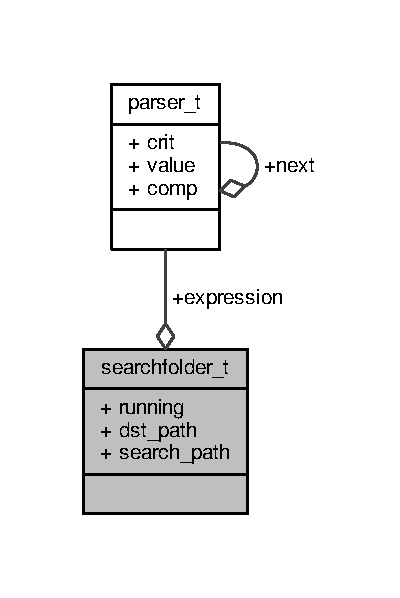
\includegraphics[width=185pt]{structsearchfolder__t__coll__graph}
\end{center}
\end{figure}
\subsection*{Data Fields}
\begin{DoxyCompactItemize}
\item 
bool {\bfseries running}\hypertarget{structsearchfolder__t_a36f7b6be7108281af77939ceaec42fd6}{}\label{structsearchfolder__t_a36f7b6be7108281af77939ceaec42fd6}

\item 
char $\ast$ {\bfseries dst\+\_\+path}\hypertarget{structsearchfolder__t_a74a7cec2bc63610109c58ef392d14e27}{}\label{structsearchfolder__t_a74a7cec2bc63610109c58ef392d14e27}

\item 
char $\ast$ {\bfseries search\+\_\+path}\hypertarget{structsearchfolder__t_a614ce96a64fa528698e05ce10070efe9}{}\label{structsearchfolder__t_a614ce96a64fa528698e05ce10070efe9}

\item 
\hyperlink{structparser__t}{parser\+\_\+t} $\ast$ {\bfseries expression}\hypertarget{structsearchfolder__t_a37eed245f4d8beb45412f8ba904643b2}{}\label{structsearchfolder__t_a37eed245f4d8beb45412f8ba904643b2}

\end{DoxyCompactItemize}


\subsection{Detailed Description}


Definition at line 11 of file searchfolder.\+c.



The documentation for this struct was generated from the following file\+:\begin{DoxyCompactItemize}
\item 
/home/claudio/git/smart-\/folder/src/searchfolder.\+c\end{DoxyCompactItemize}

\chapter{File Documentation}
\hypertarget{validator_8h}{}\section{validator.\+h File Reference}
\label{validator_8h}\index{validator.\+h@{validator.\+h}}


Validates files against a parsed criteria expression.  


{\ttfamily \#include $<$stdbool.\+h$>$}\\*
{\ttfamily \#include $<$sys/stat.\+h$>$}\\*
{\ttfamily \#include \char`\"{}parser.\+h\char`\"{}}\\*
Include dependency graph for validator.\+h\+:\nopagebreak
\begin{figure}[H]
\begin{center}
\leavevmode
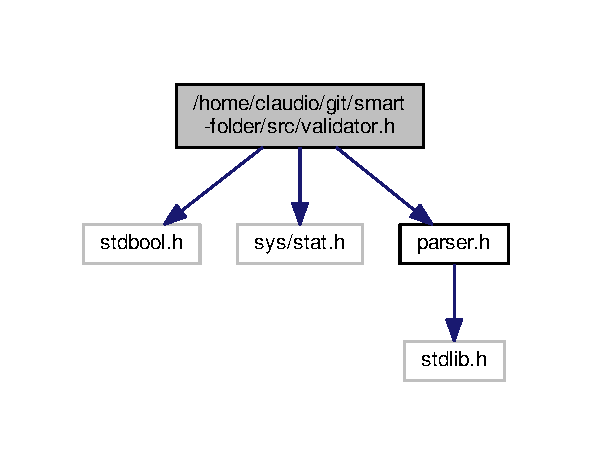
\includegraphics[width=284pt]{validator_8h__incl}
\end{center}
\end{figure}
This graph shows which files directly or indirectly include this file\+:
\nopagebreak
\begin{figure}[H]
\begin{center}
\leavevmode
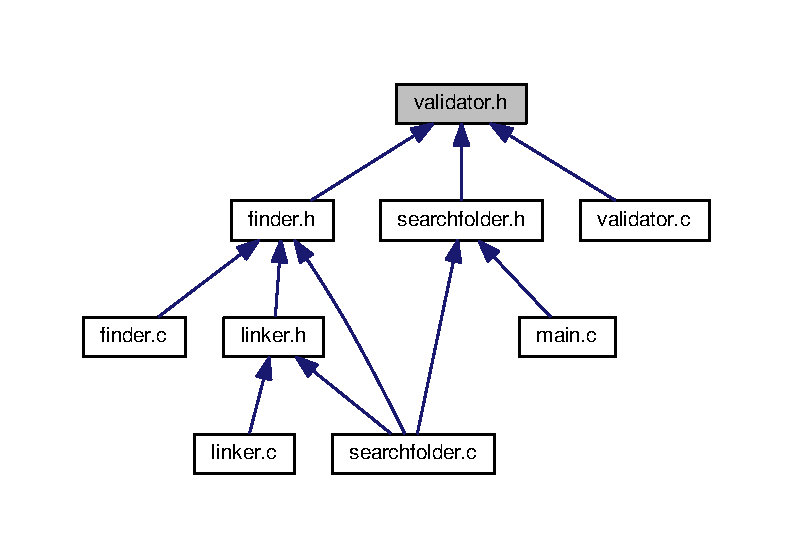
\includegraphics[width=350pt]{validator_8h__dep__incl}
\end{center}
\end{figure}
\subsection*{Functions}
\begin{DoxyCompactItemize}
\item 
bool \hyperlink{validator_8h_a0abc93342b9898145ea067c4a538022a}{validator\+\_\+validate} (char $\ast$filename, struct stat $\ast$filestat, \hyperlink{structparser__t}{parser\+\_\+t} $\ast$expression)
\begin{DoxyCompactList}\small\item\em Validates a file against an expression. \end{DoxyCompactList}\end{DoxyCompactItemize}


\subsection{Detailed Description}
Validates files against a parsed criteria expression. 



\subsection{Function Documentation}
\index{validator.\+h@{validator.\+h}!validator\+\_\+validate@{validator\+\_\+validate}}
\index{validator\+\_\+validate@{validator\+\_\+validate}!validator.\+h@{validator.\+h}}
\subsubsection[{\texorpdfstring{validator\+\_\+validate(char $\ast$filename, struct stat $\ast$filestat, parser\+\_\+t $\ast$expression)}{validator_validate(char *filename, struct stat *filestat, parser_t *expression)}}]{\setlength{\rightskip}{0pt plus 5cm}bool validator\+\_\+validate (
\begin{DoxyParamCaption}
\item[{char $\ast$}]{filename, }
\item[{struct stat $\ast$}]{filestat, }
\item[{{\bf parser\+\_\+t} $\ast$}]{exp}
\end{DoxyParamCaption}
)}\hypertarget{validator_8h_a0abc93342b9898145ea067c4a538022a}{}\label{validator_8h_a0abc93342b9898145ea067c4a538022a}


Validates a file against an expression. 


\begin{DoxyParams}{Parameters}
{\em filename} & The file\textquotesingle{}s name \\
\hline
{\em filestat} & The file\textquotesingle{}s attributes \\
\hline
{\em expression} & The expression used to validate the file \\
\hline
\end{DoxyParams}
\begin{DoxyReturn}{Returns}
If the file is valid
\end{DoxyReturn}


Definition at line 179 of file validator.\+c.


%--- End generated contents ---

% Index
\backmatter
\newpage
\phantomsection
\clearemptydoublepage
\addcontentsline{toc}{chapter}{Index}
\printindex

\end{document}
